\chapter{Blockchain}

\chapterquote{Blockchain is the technology that allows trust without trusting.}{Vitalik Buterin \cite{Buterin2014Ethereum}}

\section*{Introduction}
\addcontentsline{toc}{section}{Introduction}

The blockchain payment integration represents a crucial component of the Korpor platform, focusing on secure investor payment processing and transparent transaction recording \cite{Nakamoto2008Bitcoin}. This sprint implements a hybrid approach combining traditional payment gateways with blockchain technology to ensure both user convenience and transaction security.

The main feature centers on investor payment flows where users can securely invest in real estate projects through Paymee payment gateway, with all transactions automatically recorded on the blockchain for transparency and immutability \cite{Tapscott2016Blockchain}. This integration provides investors with traditional payment convenience while leveraging blockchain's security and transparency benefits.

\section{Sprint 7: Blockchain Payment Integration}

\subsection{Analysis}
\subsubsection{Use Cases Overview}

The blockchain integration within the \textbf{\textcolor{primary}{Korpor}} platform addresses four core functionalities: \textbf{Investment Recording} for immutable ownership proof, \textbf{Project Registration} for on-chain project verification, \textbf{Rent Distribution} for automated fair payout calculation, and \textbf{Transaction Verification} for comprehensive audit trails and regulatory compliance.

\subsubsection{Objectives of Integration}

The blockchain integration enhances the platform through three key objectives: \textbf{Security and trust} via cryptographically signed transactions \cite{Zheng2018BlockchainChallenges}, \textbf{Decentralization and immutability} ensuring data cannot be altered \cite{Antonopoulos2018MasteringEthereum}, and \textbf{Smart contract automation} for efficient business logic execution \cite{Bartoletti2017EmpiricalAnalysis}.

\subsubsection{Use Case Diagram}

The transaction management  system serves as the core component for handling all blockchain-based investment activities within the Korpor platform. Figure \ref{fig:transaction-use-case} illustrates the main use cases for blockchain transaction management, showing how the system automatically saves all transactions as immutable smart contracts.

\begin{figure}[htbp]
    \centering
    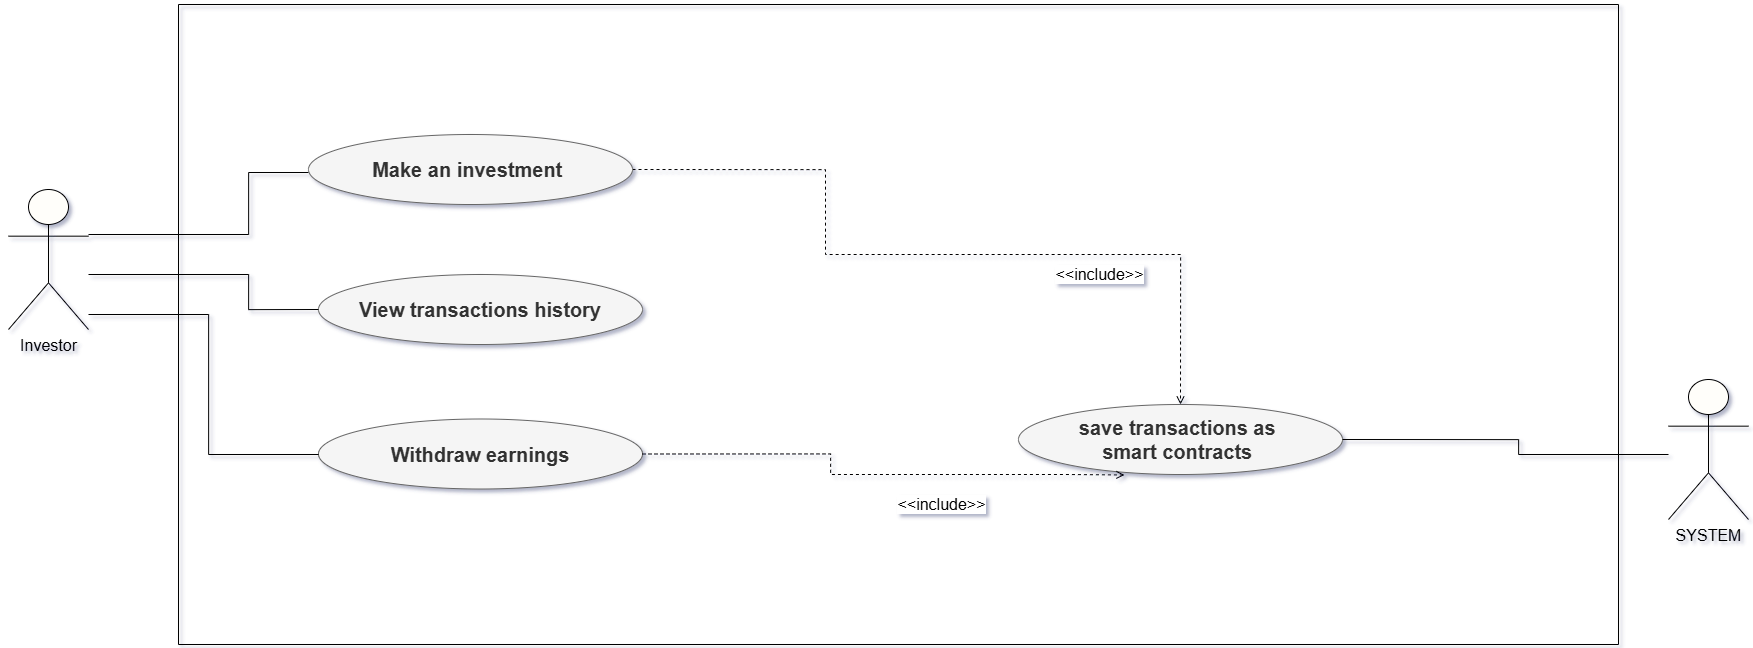
\includegraphics[width=0.8\textwidth]{images/transaction_use_case_diagram.png}
    \caption{Blockchain Transaction Management Use Case Diagram}
    \label{fig:transaction-use-case}
\end{figure}
\subsubsection{Textual Use Case Descriptions}

\begin{table}[htbp]
    \centering
    \begin{tabular}{|p{3cm}|p{10cm}|}
        \hline
        \textbf{Use Case} & \textbf{Make an Investment} \\
        \hline
        \textbf{Actor} & Investor \\
        \hline
        \textbf{Precondition} & Investor is authenticated and has sufficient funds \\
        \hline
        \textbf{Main Scenario} & Investor selects a property and initiates investment through secure payment processing \\
        \hline
        \textbf{Postcondition} & Investment is recorded on blockchain and investor receives confirmation \\
        \hline
    \end{tabular}
    \caption{Make Investment Transaction Use Case Description}
    \label{tab:make-investment-use-case}
\end{table}

\begin{table}[htbp]
    \centering
    \begin{tabular}{|p{3cm}|p{10cm}|}
        \hline
        \textbf{Use Case} & \textbf{View Transactions History} \\
        \hline
        \textbf{Actor} & Investor \\
        \hline
        \textbf{Precondition} & Investor is authenticated and has previous transactions \\
        \hline
        \textbf{Main Scenario} & Investor accesses comprehensive transaction history with blockchain verification \\
        \hline
        \textbf{Postcondition} & Complete transaction timeline is displayed with verifiable blockchain records \\
        \hline
    \end{tabular}
    \caption{View Transaction History Use Case Description}
    \label{tab:view-transactions-use-case}
\end{table}
\newpage
\begin{table}[htbp]
    \centering
    \begin{tabular}{|p{3cm}|p{10cm}|}
        \hline
        \textbf{Use Case} & \textbf{Withdraw Earnings} \\
        \hline
        \textbf{Actor} & Investor \\
        \hline
        \textbf{Precondition} & Investor has available earnings from property investments \\
        \hline
        \textbf{Main Scenario} & Investor requests withdrawal and system processes payment securely \\
        \hline
        \textbf{Postcondition} & Earnings are transferred and withdrawal is recorded on blockchain \\
        \hline
    \end{tabular}
    \caption{Withdraw Earnings Transaction Use Case Description}
    \label{tab:withdraw-earnings-use-case}
\end{table}

\begin{table}[htbp]
    \centering
    \begin{tabular}{|p{3cm}|p{10cm}|}
        \hline
        \textbf{Use Case} & \textbf{Save Transactions as Smart Contracts} \\
        \hline
        \textbf{Actor} & System \\
        \hline
        \textbf{Precondition} & Transaction has been initiated and validated \\
        \hline
        \textbf{Main Scenario} & System automatically records transaction details in immutable smart contracts \\
        \hline
        \textbf{Postcondition} & Transaction is permanently stored on blockchain for transparency and audit \\
        \hline
    \end{tabular}
    \caption{Save Transactions as Smart Contracts Use Case Description}
    \label{tab:save-transactions-use-case}
\end{table}

\subsection{Modeling}

The blockchain component is designed to integrate seamlessly within the overall architecture of the \textbf{\textcolor{primary}{Korpor}} platform. This section outlines how the blockchain fits into the system and the technologies used for its implementation.

\begin{itemize}
    \item \textbf{How blockchain fits into the overall system architecture}
    \begin{itemize}
        \item The backend communicates with smart contracts deployed on the Ethereum blockchain.
        \item Transactions such as investments, project registrations, and rent distributions are processed and recorded on-chain.
        \item The blockchain acts as a complementary layer to ensure data integrity and traceability.
    \end{itemize}

    \item \textbf{On-chain vs off-chain components}
    \begin{itemize}
        \item \textit{On-chain:}
        \begin{itemize}
            \item Smart contracts handle investments, project registrations, and rent distributions.
            \item Data recorded on-chain is immutable and publicly verifiable.
        \end{itemize}
        \item \textit{Off-chain:}
        \begin{itemize}
            \item User data, authentication, and detailed analytics are managed by the backend and stored in a centralized database (MySQL).
            \item Interaction with the blockchain is facilitated through API endpoints and external services \cite{Xu2019ArchitectingBlockchainApplications}.
        \end{itemize}
    \end{itemize}

\end{itemize}

\subsection{Implementation}
\subsubsection{Technologies Used}
The blockchain implementation utilizes several key technologies:

\begin{itemize}
    \item \textbf{Solidity:} Smart contract programming language for Ethereum blockchain \cite{SolidityDocs}
    \item \textbf{Ethers.js:} JavaScript library for blockchain interaction \cite{EthersJSDocs}
    \item \textbf{Sepolia Testnet:} Ethereum test network for safe development
    \item \textbf{Infura:} Cloud-based Ethereum node access \cite{InfuraWeb3}
    \item \textbf{MetaMask:} Cryptocurrency wallet for decentralized applications \cite{MetaMaskDocs}
\end{itemize}

\subsubsection{Third-Party Payment Integration: Paymee}

In the Korpor platform, secure and reliable payment processing is fundamental to enabling users to invest in real estate projects with confidence. While blockchain handles transparency and decentralization for on-chain interactions, fiat payments from users need to be handled via trusted third-party providers. For this purpose, we chose \textbf{Paymee} as our main payment gateway.

% Placeholder for Paymee Framework diagram
% \begin{figure}[htbp]
% \centering
% 
\includegraphics[width=0.8\textwidth]{images/paymee_framework.png}
% \caption{Paymee Framework}
% \label{fig:paymee-framework}
% \end{figure}

\subsubsection{Role of Paymee in the Architecture}

Paymee acts as a bridge between the user's traditional banking system and our decentralized investment platform. When a user decides to invest in a project, the fiat transaction is processed securely via Paymee. Upon confirmation, the platform triggers an on-chain event that records the investment using a smart contract, ensuring both real-world and blockchain-level consistency.

\begin{itemize}
    \item Paymee provides a secure and verified method for processing payments via bank cards or wallets.
    \item It offers real-time transaction status updates, which are essential for synchronizing with blockchain confirmations.
    \item The integration ensures that only successful payments are recorded on-chain, reducing fraud and improving traceability \cite{Bamakan2020BlockchainPayment}.
\end{itemize}

\subsubsection{Justifying the Choice of Paymee}

Several third-party payment providers are available in Tunisia, including  \textbf{Flouci} 
\includegraphics[width=0.05\textwidth]{images/icons/flouci_icon.png} and  \textbf{Konnect} 
\includegraphics[width=0.05\textwidth]{images/icons/konnect_icon.png} , however, \textbf{Paymee} was chosen due to its distinct advantages in several key areas:

\begin{itemize}
  \item \textbf{Regulatory Compliance:} Fully compliant with local regulations and has established partnerships with most major Tunisian banks.
  
  \item \textbf{Developer Experience:} Offers clear documentation, a stable sandbox environment, and responsive customer support.
  
  \item \textbf{Payment Mode:} Supports a wide range of payment methods, including both local and international options.
  
  \item \textbf{Pricing:} Offers simplified and transparent pricing with competitive rates.
  
  \item \textbf{User Experience:} Provides a minimalistic and intuitive user interface that reduces drop-off rates during transactions.
  
  \item \textbf{Flexibility:} Highly flexible and easily integrates into diverse use cases, adapting to the requirements of individual investors.
\end{itemize}
\newpage
% Placeholder for Payment Providers Comparison Table
\begin{table}[htbp]
\centering
\caption{Comparison of Payment Providers: Paymee vs Flouci vs Konnect}
\label{tab:payment_comparison}
\begin{tabular}{|p{4cm}|p{3.5cm}|p{3.5cm}|p{3.5cm}|}
\hline
\textbf{Feature} & \textbf{Paymee} & \textbf{Flouci} & \textbf{Konnect} \\ \hline
\textbf{Regulatory Compliance} & Fully compliant with local regulations & Limited compliance & Enterprise-focused, may have specific requirements \\ \hline
\textbf{Developer Experience} & Clear documentation, stable sandbox, responsive support & Less stable APIs, limited documentation & Lengthy onboarding, limited flexibility \\ \hline
\textbf{Payment Model} & Ideal for recurring, high-trust investments & Not suited for investment models & Enterprise-focused with fixed pricing \\ \hline
\textbf{Pricing} & Simplified and transparent & Unclear pricing structure & Complex pricing and fees \\ \hline
\textbf{User Experience} & Minimalistic UI, reliable webhooks, low drop-offs & Less reliable, mobile payment focus & Enterprise UI, longer process, limited customization \\ \hline
\textbf{Flexibility} & High flexibility in fee structures & Low flexibility & Low flexibility, rigid fee structures \\ \hline
\end{tabular}
\end{table}

Based on these factors, \textbf{Paymee} was selected as the most suitable payment provider for the Korpor platform, playing a pivotal role in bridging traditional finance with our blockchain-based investment infrastructure.

\subsubsection{Smart Contract Design}

\paragraph{Smart Contracts Overview}

A smart contract is a self-executing contract with the terms of the agreement directly written into lines of code \cite{Szabo1997SmartContracts}. These contracts run on blockchain platforms, such as Ethereum, and are designed to automatically enforce and execute the terms of an agreement without the need for intermediaries. 

Smart contracts operate on decentralized networks, ensuring transparency, immutability, and security. They allow parties to interact and transact with one another in a trustless environment, where the contract's logic is executed automatically when predefined conditions are met \cite{Wohrer2018SmartContractApplications}.

\paragraph{Smart Contract Responsibilities}

The smart contract in the Korpor application is responsible for managing the critical aspects of the platform. The main responsibilities include:

\begin{itemize}
    \item \textbf{Recording Investments:} The smart contract records each user's investment when they invest in a project.
    \item \textbf{Project Registration:} Real estate companies can register new projects.
    \item \textbf{Rent Distribution:} The contract ensures that rental income is distributed fairly to investors.
    \item \textbf{Transaction Verification:} All actions taken within the contract are securely logged on the blockchain.
\end{itemize}

\paragraph{Data Structures and Functions}

In the smart contract, several data structures and functions are employed to manage and store key information, facilitating efficient interaction with the system \cite{Dannen2017SoliditySmartContracts}.

\subsubsection{Data Structures}

The contract uses `structs` to represent complex data types like project and investor details.

\paragraph{Project Struct:}
The `Project` struct stores the details of each project:
\begin{verbatim}
struct Project {
    uint256 projectId;
    string projectName;
    address companyAddress;
    uint256 totalFunding;
    uint256 rentIncome;
    uint256 numInvestors;
}
\end{verbatim}

\paragraph{Investor Struct:}
The investor struct stores individual investment details for tracking purposes.
\newpage
\subsubsection*{Mobile Payment Interface}

The mobile application provides a seamless interface for investors to manage their blockchain-based transactions. Figure \ref{fig:mobile-payment-interface} demonstrates the complete mobile payment workflow including investment initiation, payment processing, and withdrawal functionality.

% \begin{figure}[htbp]
%     \centering
%     % Three mobile interface images side by side
%     \begin{subfigure}[b]{0.3\textwidth}
%         \centering
%         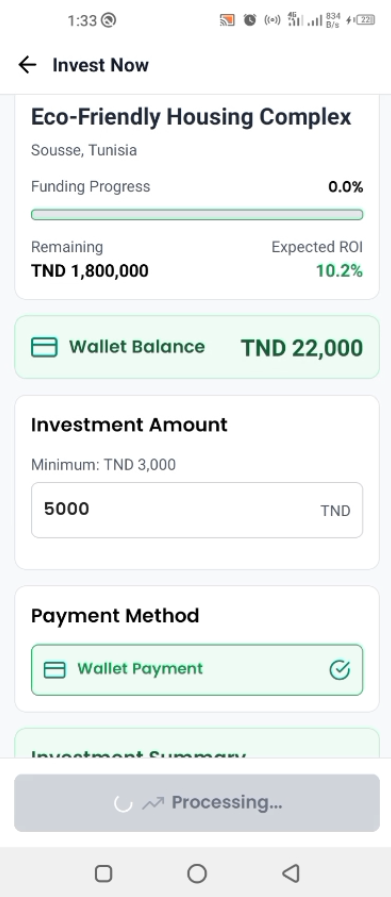
\includegraphics[width=\textwidth]{images/mobile_invest_interface.png}
%         \caption{Investment Interface}
%         \label{fig:mobile-invest}
%     \end{subfigure}
%     \hfill
%     \begin{subfigure}[b]{0.3\textwidth}
%         \centering
%         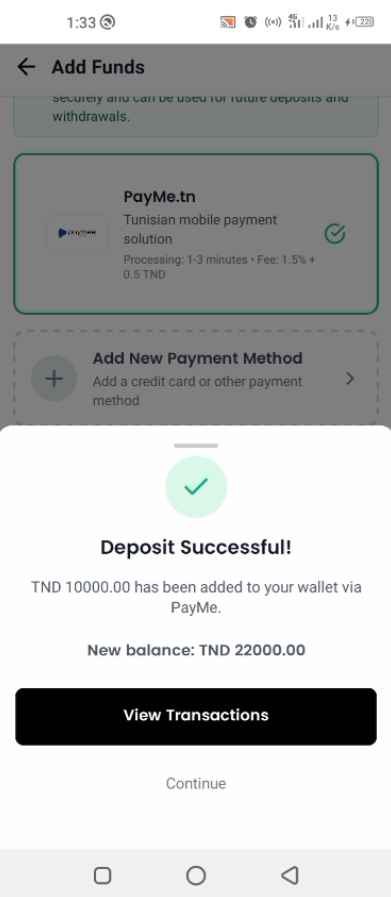
\includegraphics[width=\textwidth]{images/mobile_payment_process.png}
%         \caption{Payment Process}
%         \label{fig:mobile-payment}
%     \end{subfigure}
%     \hfill
%     \begin{subfigure}[b]{0.3\textwidth}
%         \centering
%         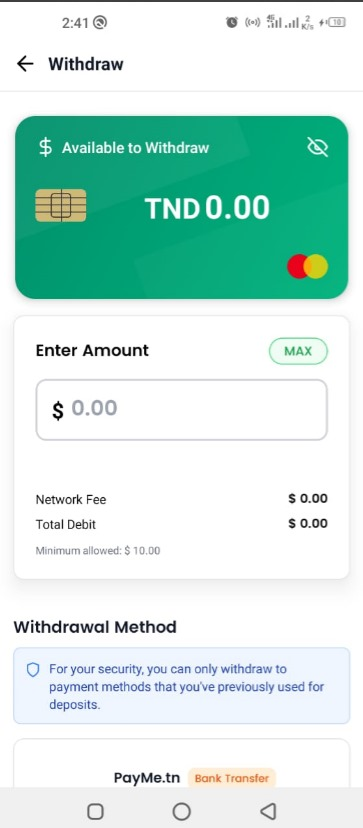
\includegraphics[width=\textwidth]{images/mobile_withdraw_interface.png}
%         \caption{Withdrawal Interface}
%         \label{fig:mobile-withdraw}
%     \end{subfigure}
%     \caption{Mobile Payment Interface: Investment, Payment, and Withdrawal Process}
%     \label{fig:mobile-payment-interface}
% \end{figure}


\subsubsection*{Admin Blockchain Visualization}

The super admin dashboard provides comprehensive visualization and management capabilities for blockchain smart contracts. Figure \ref{fig:admin-blockchain-visualization} shows the administrative interface for monitoring and managing blockchain transactions and smart contract interactions.

% \begin{figure}[htbp]
%     \centering
%     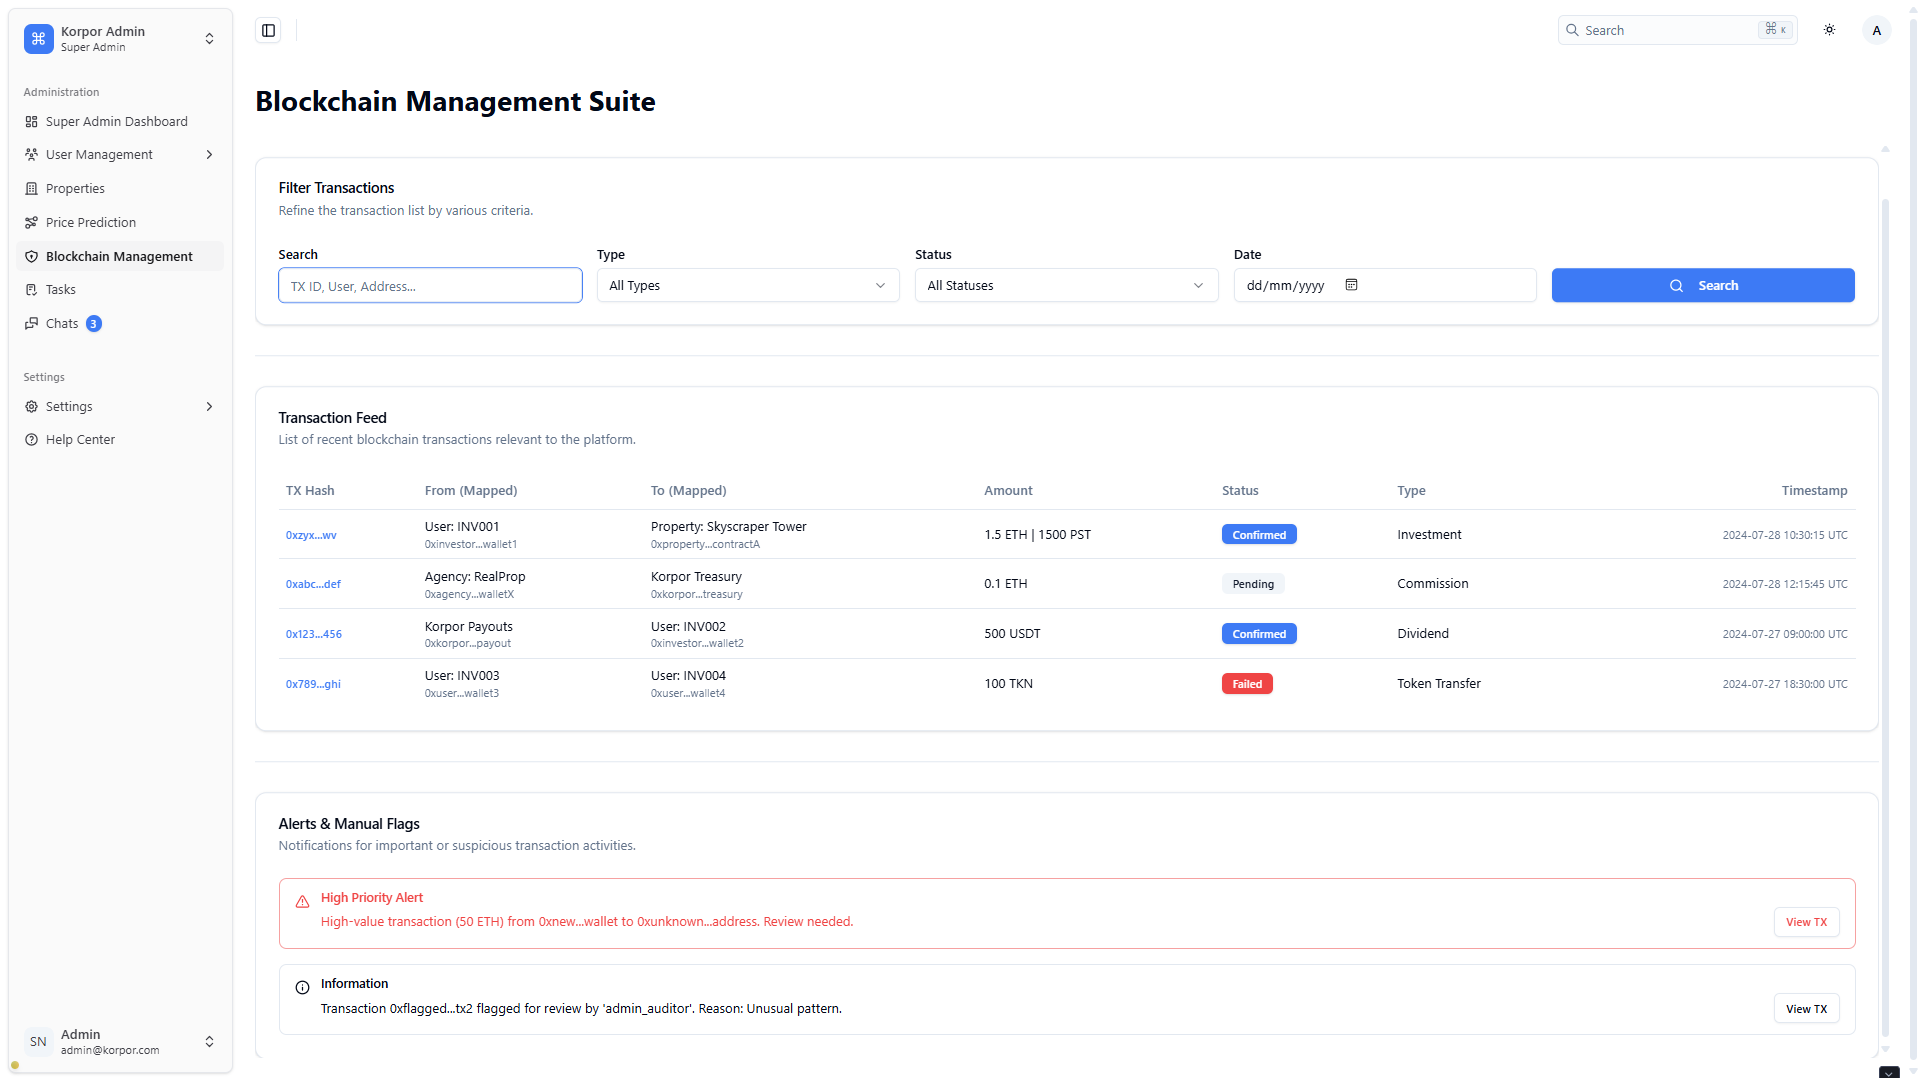
\includegraphics[width=0.8\textwidth]{images/admin_blockchain_dashboard.png}
%     \caption{Super Admin Blockchain Smart Contract Visualization Dashboard}
%     \label{fig:admin-blockchain-visualization}
% \end{figure}
% \newpage

\subsection{Test}
\subsubsection{Transaction Flow Testing}

The blockchain payment integration was thoroughly tested through a complete end-to-end transaction flow, demonstrating the seamless integration between Paymee payment gateway and blockchain recording. The following test scenario validates the entire investment process:

\paragraph{ Initiate New Transaction}
The investor initiates a new investment transaction through the platform interface, selecting the desired property and investment amount.

\begin{figure}[htbp]
    \centering
    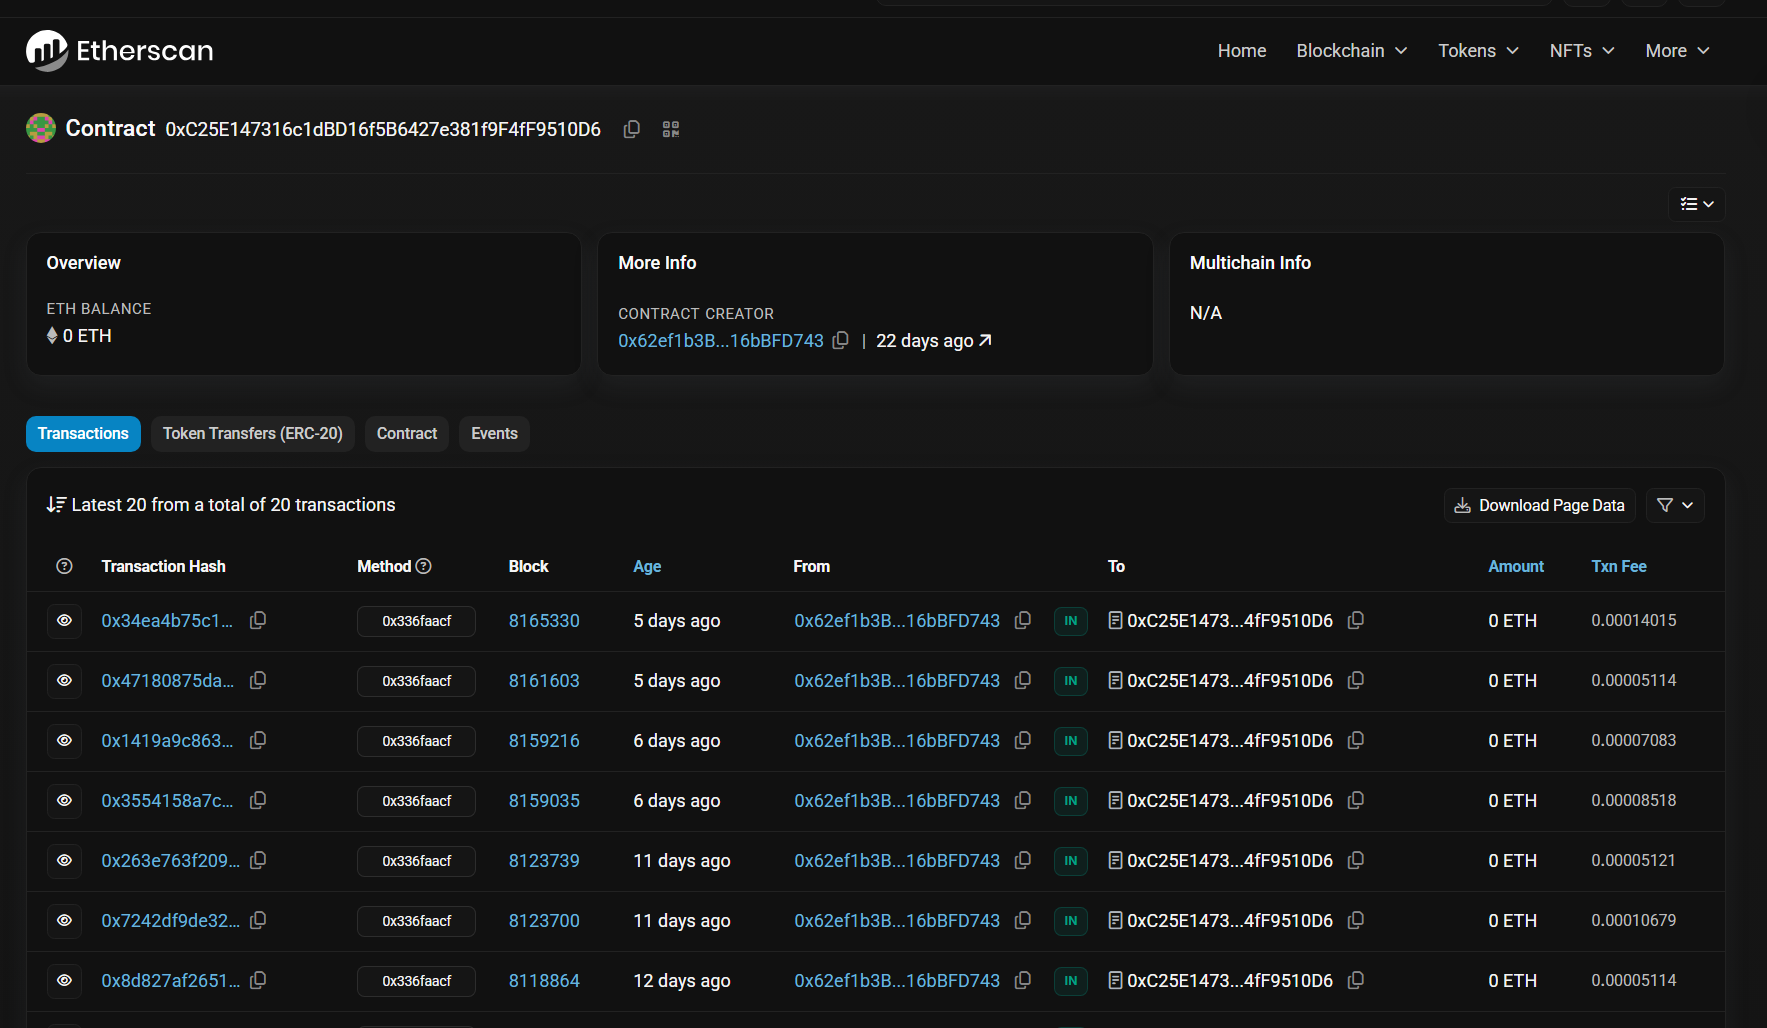
\includegraphics[width=0.8\textwidth]{images/new_transaction_init.png}
    \caption{New Transaction Initiation Interface}
    \label{fig:new-transaction-init}
\end{figure}


\paragraph{ Database Transaction Recording}
Upon payment initiation, the transaction information is immediately saved to the database with a "pending" status, ensuring proper tracking of the investment process.

\begin{figure}[htbp]
    \centering
    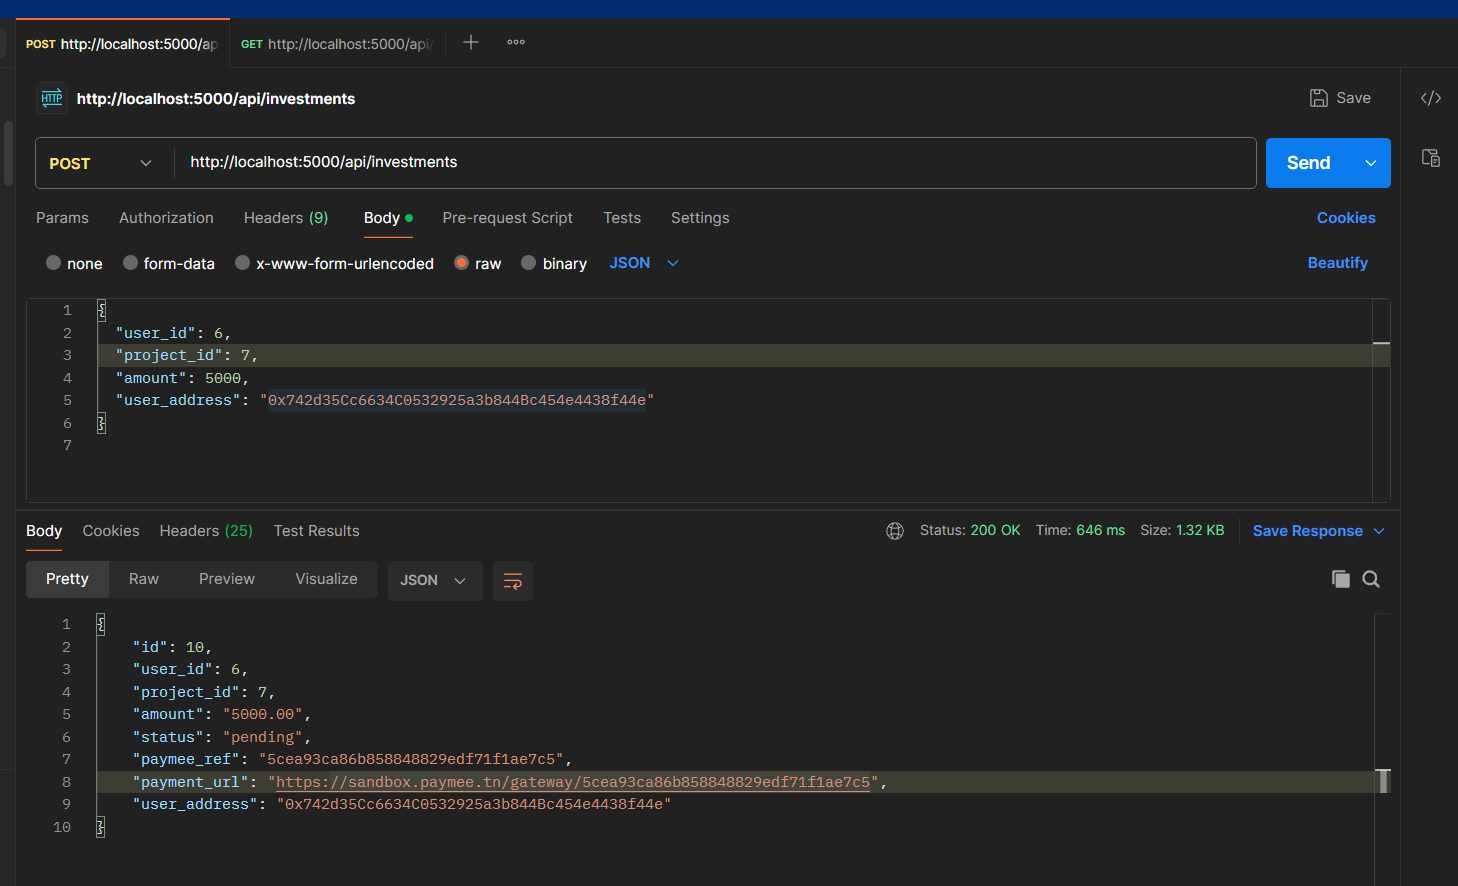
\includegraphics[width=0.8\textwidth]{images/transaction_pending_status.png}
    \caption{Transaction Saved with Pending Status}
    \label{fig:transaction-pending-status}
\end{figure}

\newpage

\paragraph{Payment Confirmation and Blockchain Recording}
After successful payment confirmation, the Paymee callback is executed, triggering the blockchain investment recording process. The system generates a transaction hash confirming the successful blockchain entry.

\begin{figure}[htbp]
    \centering
    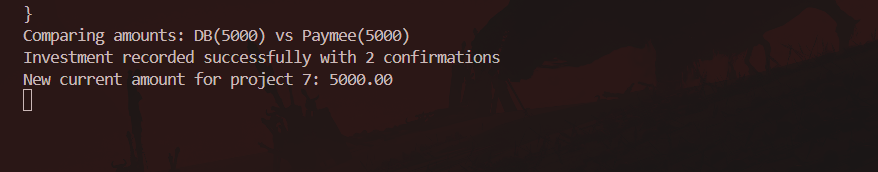
\includegraphics[width=0.8\textwidth]{images/payment_confirmation_success.png}
    \caption{Payment Confirmation Success Message}
    \label{fig:payment-confirmation-success}
\end{figure}

\begin{figure}[htbp]
    \centering
    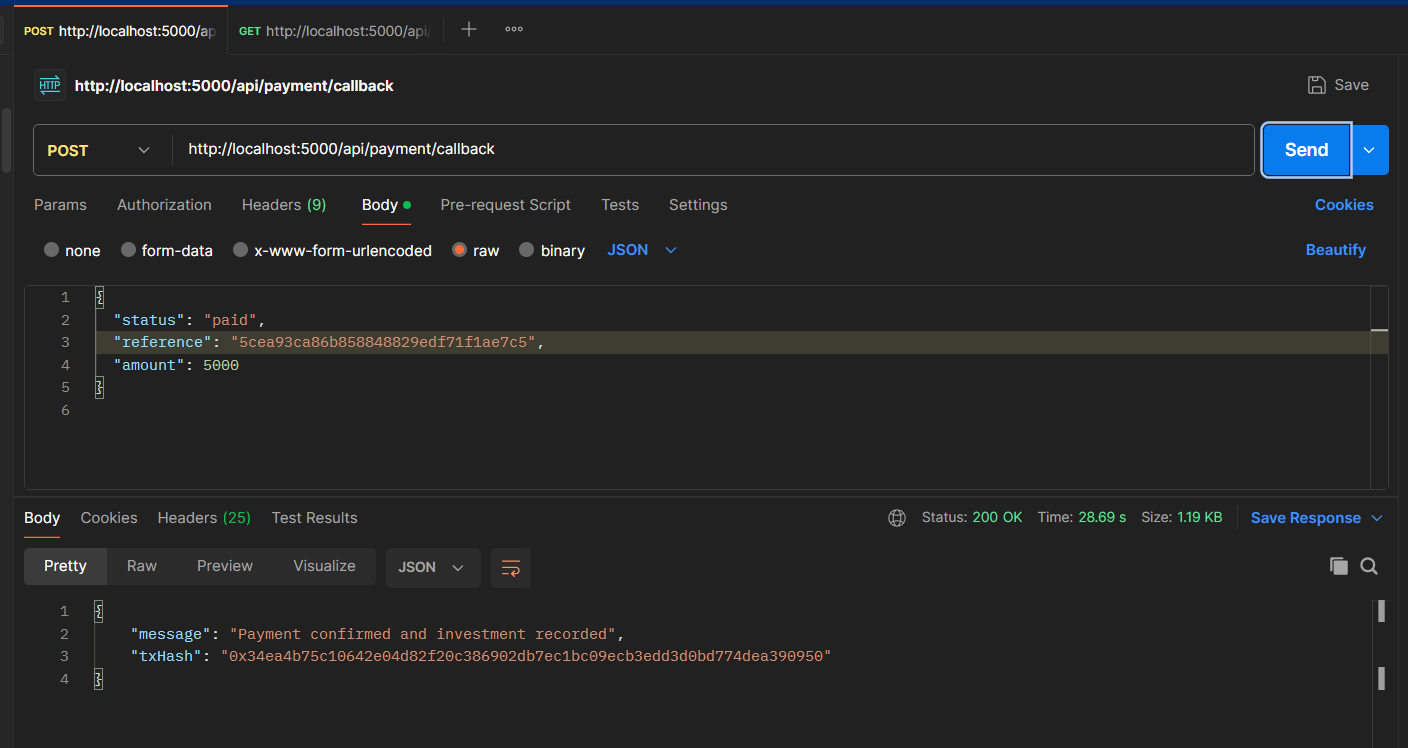
\includegraphics[width=0.9\textwidth]{images/blockchain_hash_generated.png}
    \caption{Blockchain Transaction Hash Generated}
    \label{fig:blockchain-hash-generated}
\end{figure}

\newpage
\paragraph{Transaction Status Update}
The investment status is updated to "confirmed" in the database, the current investment amount is adjusted, and the blockchain record hash is permanently stored for future reference and verification.

\begin{figure}[htbp]
    \centering
    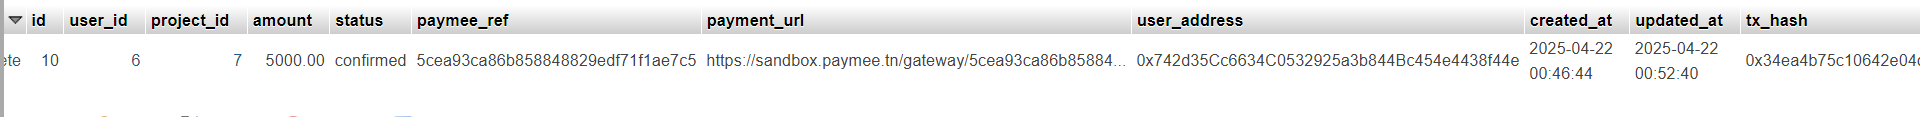
\includegraphics[width=1\textwidth]{images/transaction_confirmed_status.png}
    \caption{Transaction Status Updated to Confirmed}
    \label{fig:transaction-confirmed-status}
\end{figure}

\paragraph{Blockchain Verification}
The transaction is successfully recorded on the Ethereum Sepolia testnet, providing immutable proof of the investment that can be independently verified through Etherscan.

\begin{figure}[htbp]
    \centering
    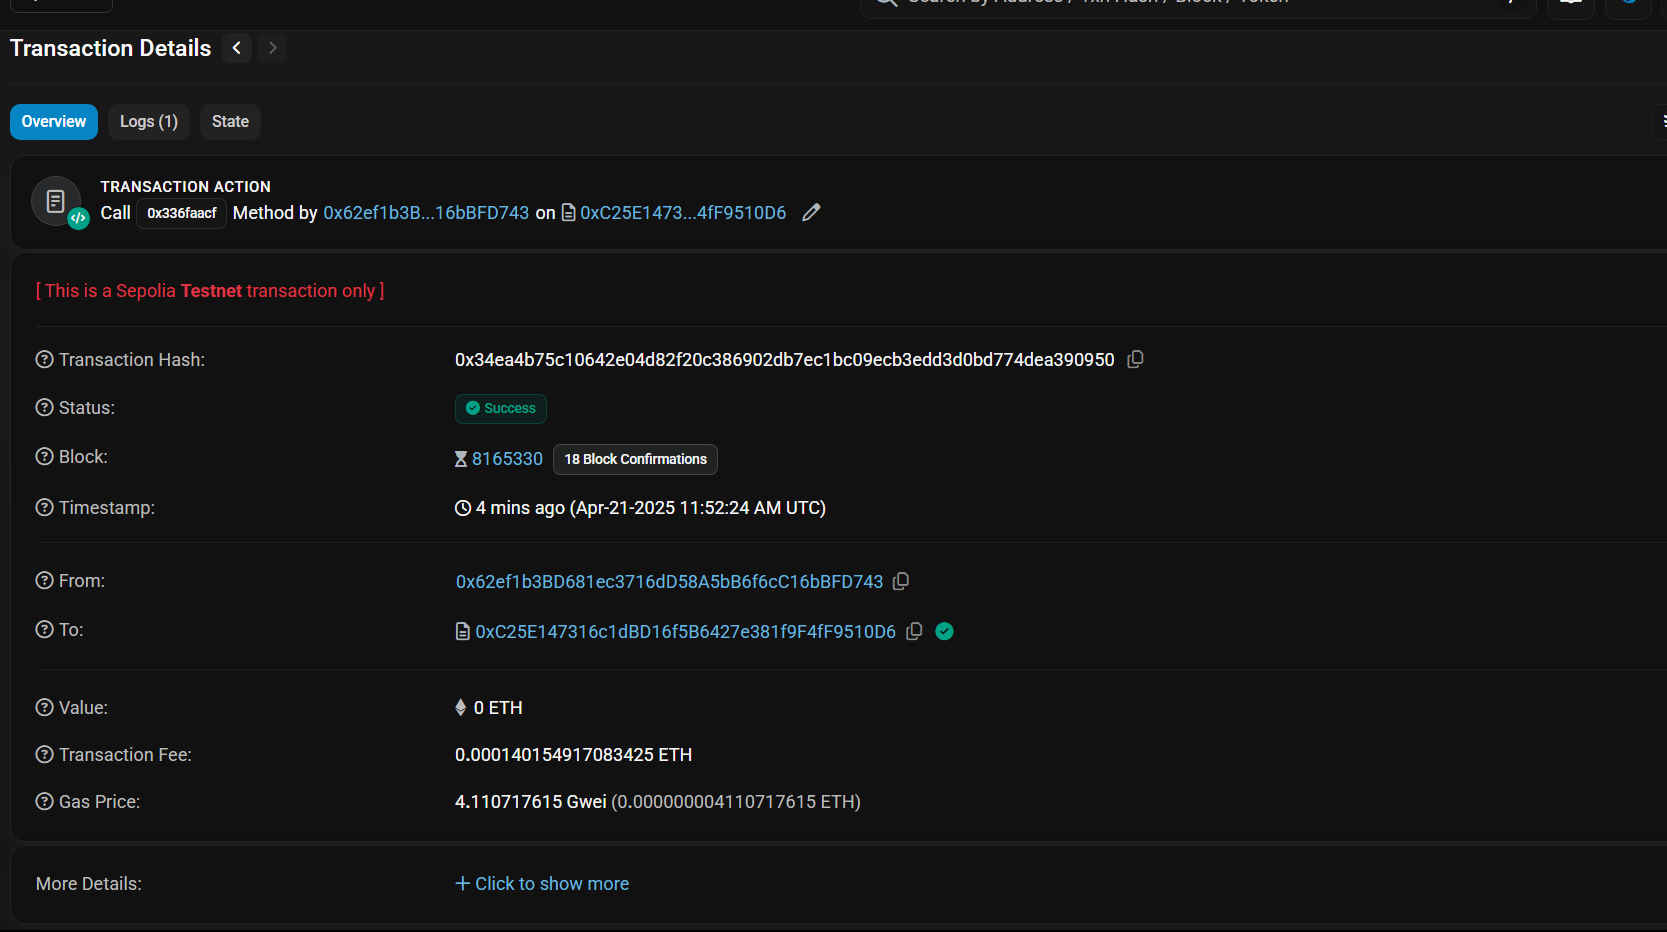
\includegraphics[width=0.9\textwidth]{images/etherscan_blockchain_record.png}
    \caption{Transaction Record on Etherscan Sepolia Blockchain}
    \label{fig:etherscan-blockchain-record}
\end{figure}

\subsubsection{Smart Contract Validation}
Smart contract functions were thoroughly tested on the Sepolia testnet, validating investment recording, project registration, and rent distribution mechanisms. All test scenarios passed successfully, confirming the reliability of the blockchain implementation and the seamless integration with the Paymee payment gateway.
\newpage
\subsection{Retrospective}

The blockchain integration sprint successfully delivered secure payment processing and transparent transaction recording. Table \ref{tab:blockchain-retrospective} summarizes the key achievements and future improvements.

\begin{table}[htbp]
    \centering
    \begin{tabular}{|p{3cm}|p{10cm}|}
        \hline
        \textbf{Category} & \textbf{Details} \\
        \hline
        \textbf{What Went Well} & 
        \begin{itemize}
            \item Successfully integrated Paymee payment gateway with blockchain
            \item Achieved secure and transparent investment recording
            \item Smart contracts deployed and tested successfully on Sepolia
            \item Payment flow validation completed without major issues
        \end{itemize} \\
        \hline
        \textbf{Action Items} & 
        \begin{itemize}
            \item Implement gas optimization for smart contract operations
            \item Add automated monitoring for transaction failures
        \end{itemize} \\
        \hline
    \end{tabular}
    \caption{Blockchain Integration Sprint Retrospective Summary}
    \label{tab:blockchain-retrospective}
\end{table}